\documentclass[lualatex,ja=standard,a4paper,12pt]{bxjsarticle}
\usepackage{amsmath, amssymb, amsthm, bm}
\usepackage{geometry}
\usepackage{xcolor}
\usepackage{tcolorbox}
\usepackage{booktabs}
\usepackage{array}
\usepackage{tikz}
\usetikzlibrary{positioning, arrows.meta, fit}

\geometry{margin=25mm}

\tcbuselibrary{theorems, skins, breakable}

\newtcolorbox{defbox}[1]{
  colback=blue!5, colframe=blue!60!black,
  fonttitle=\bfseries, title={#1}, arc=3pt, breakable
}
\newtcolorbox{thmbox}[1]{
  colback=green!5, colframe=green!50!black,
  fonttitle=\bfseries, title={#1}, arc=3pt, breakable
}
\newtcolorbox{pointbox}{
  colback=orange!8, colframe=orange!70!black,
  fonttitle=\bfseries, title={ポイント}, arc=3pt, breakable
}
\newtcolorbox{exbox}[1]{
  colback=gray!6, colframe=gray!50,
  fonttitle=\bfseries, title={例：#1}, arc=3pt, breakable
}
\newtcolorbox{derivbox}{
  colback=purple!4, colframe=purple!50!black,
  fonttitle=\bfseries, title={導出}, arc=3pt, breakable
}
\newtcolorbox{warningbox}{
  colback=red!5, colframe=red!60!black,
  fonttitle=\bfseries, title={注意}, arc=3pt, breakable
}
\newtcolorbox{algobox}[1]{
  colback=cyan!4, colframe=cyan!50!black,
  fonttitle=\bfseries, title={#1}, arc=3pt, breakable
}

\newcommand{\mvn}{\mathrm{MVN}}
\newcommand{\IW}{\mathrm{inverse\text{-}Wishart}}
\newcommand{\IG}{\mathrm{inverse\text{-}gamma}}

\title{{\large Hoff 第11章} \\[6pt]
       \textbf{Linear and Generalized Linear Mixed Effects Models} \\[4pt]
       {\normalsize （線形・一般化線形混合効果モデル）ゼミ資料}}
\author{}
\date{}

\begin{document}
\maketitle
\thispagestyle{empty}

% ===========================
\section{この章のモチベーション}
% ===========================

第8章では，複数のグループ（学校など）それぞれに複数の観測があるデータに対して
\textbf{階層モデル}を導入した．そこでは
\begin{itemize}
  \item グループ内：$Y_{i,j} \sim \mathrm{Normal}(\theta_j, \sigma^2)$（グループ内のバラつき）
  \item グループ間：$\theta_1, \ldots, \theta_m \sim \mathrm{Normal}(\mu, \tau^2)$（グループ平均のバラつき）
\end{itemize}
という2段構えで，グループごとの\textbf{平均}を推定した．

\medskip
\noindent\textbf{この章の問い：}
グループごとに違うのが「平均」だけでなく，
\textbf{変数間の関係（回帰係数）}だったらどうするか？

\medskip
\noindent 答えは素直で，第8章の階層モデルの「平均」を「回帰係数ベクトル」に置き換えればよい．

\begin{center}
\small
\renewcommand{\arraystretch}{1.5}
\setlength{\tabcolsep}{4pt}
\begin{tabular}{lll}
\toprule
 & 第8章（階層正規モデル） & 第11章（階層回帰モデル） \\
\midrule
グループ内 & $Y_{i,j} \sim \mathrm{Normal}(\theta_j, \sigma^2)$ & $Y_{i,j} \sim \mathrm{Normal}(\bm{\beta}_j^\top \bm{x}_{i,j}, \sigma^2)$ \\
グループ間 & $\theta_j \sim \mathrm{Normal}(\mu, \tau^2)$ & $\bm{\beta}_j \sim \mvn(\bm{\theta}, \Sigma)$ \\
グループ固有の量 & 平均 $\theta_j$（スカラー） & 回帰係数 $\bm{\beta}_j$（$p$次元） \\
使う道具 & 5・6章（正規，Gibbs） & 7章（多変量正規）＋9章（回帰） \\
\bottomrule
\end{tabular}
\end{center}

さらに後半では，グループ内モデルを正規回帰から
\textbf{一般化線形モデル}（ポアソン回帰など）に替えた
\textbf{一般化線形混合効果モデル}を扱う．
そこでは第10章の \textbf{Metropolis 法}と Gibbs サンプラーを組み合わせて推定する．

\begin{pointbox}
第11章は新しい道具をほとんど導入しない．
第7章（多変量正規・逆ウィシャート），第8章（階層モデル），第9章（ベイズ回帰），
第10章（Metropolis--Hastings）を\textbf{組み合わせる章}である．
各ステップが「どの章のどの結果か」を意識して読むと見通しがよい．
\end{pointbox}

% ===========================
\section{階層回帰モデル（11.1節）}
% ===========================

\subsection{動機づけ：数学の点数と SES}

\begin{exbox}{米国の公立高校の数学の点数（8.4節の続き）}
100校の10年生の数学の点数に加えて，各生徒の
\textbf{社会経済的地位（SES）}（親の収入・学歴から算出）が記録されている．
「SES が高い生徒ほど点数が高いか？　その関係は学校ごとに違うか？」を調べたい．

\medskip
\noindent\textbf{前処理：}SES を\textbf{学校ごとに中心化}する（各学校で SES の平均が0になるよう引く）．
すると回帰直線
\[
  \text{点数} \approx \beta_{1,j} + \beta_{2,j} \times \text{SES}
\]
の切片 $\beta_{1,j}$ が「学校 $j$ の平均点」，傾き $\beta_{2,j}$ が「学校 $j$ 内での SES の効果」と解釈できる．

\medskip
\noindent\textbf{まず各校で最小二乗回帰をしてみると}（教科書 Figure 11.1）：
\begin{itemize}
  \item 大半の学校で傾きは正（SES が高いほど点数が高い）だが，\textbf{負の傾きの学校もある}．
  \item \textbf{サンプルサイズが大きい学校}の推定値は全体平均の近くに集まり，
        \textbf{極端な推定値}はほとんどが\textbf{サンプルサイズの小さい学校}から出ている．
\end{itemize}
\end{exbox}

\begin{pointbox}
これは8.4節と同じ現象である：サンプルが少ないほど，たまたま偏ったデータを引いて
極端な推定値が出やすい．
対策も8章と同じで，\textbf{グループ間で情報を共有する階層モデル}によって
小さい学校の推定値を安定させる（縮小推定）．
\end{pointbox}

\subsection{モデルの定式化}

\begin{defbox}{階層正規回帰モデル}
\textbf{グループ内モデル}（学校 $j$ の中での点数のバラつき）：
\[
  Y_{i,j} = \bm{\beta}_j^\top \bm{x}_{i,j} + \epsilon_{i,j},
  \qquad
  \{\epsilon_{i,j}\} \overset{\text{i.i.d.}}{\sim} \mathrm{Normal}(0, \sigma^2). \tag{11.1}
\]
ベクトル・行列で書けば $\bm{Y}_j \sim \mvn(X_j \bm{\beta}_j,\, \sigma^2 I)$．
ここで $X_j$ は $n_j \times p$ の計画行列．
$\bm{\beta}_1, \ldots, \bm{\beta}_m, \sigma^2$ が与えられれば $\bm{Y}_1, \ldots, \bm{Y}_m$ は条件付き独立．

\medskip
\textbf{グループ間モデル}（回帰係数の学校間のバラつき）：
\[
  \bm{\beta}_1, \ldots, \bm{\beta}_m \overset{\text{i.i.d.}}{\sim} \mvn(\bm{\theta}, \Sigma). \tag{11.2}
\]

\textbf{事前分布}（すべて半共役）：
\begin{align*}
  \bm{\theta} &\sim \mvn(\bm{\mu}_0, \Lambda_0), \\
  \Sigma &\sim \IW(\eta_0, S_0^{-1}), \\
  \sigma^2 &\sim \IG(\nu_0/2,\, \nu_0\sigma_0^2/2).
\end{align*}
\end{defbox}

\noindent 数学の点数の例では $\bm{x}_{i,j} = (1, \text{SES}_{i,j})^\top$，$p = 2$ である．

\subsubsection*{グラフ表現}

\begin{center}
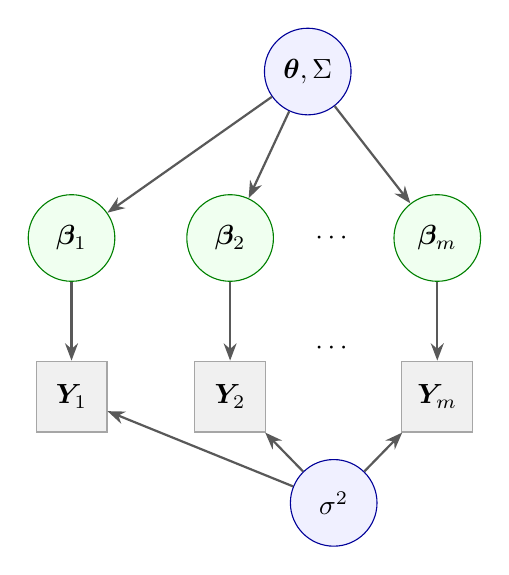
\begin{tikzpicture}[
  node distance=10mm and 9mm,
  param/.style={circle, draw=blue!60!black, fill=blue!6, minimum size=11mm, inner sep=1pt},
  grp/.style={circle, draw=green!50!black, fill=green!6, minimum size=11mm, inner sep=1pt},
  obs/.style={rectangle, draw=gray!70, fill=gray!12, minimum size=9mm, inner sep=2pt},
  arr/.style={-{Stealth[length=2.2mm]}, thick, gray!70!black}
]
  \node[param] (ts) {$\bm{\theta}, \Sigma$};
  \node[grp, below=of ts, xshift=-30mm] (b1) {$\bm{\beta}_1$};
  \node[grp, right=of b1] (b2) {$\bm{\beta}_2$};
  \node[right=4mm of b2] (bd) {$\cdots$};
  \node[grp, right=4mm of bd] (bm) {$\bm{\beta}_m$};
  \node[obs, below=of b1] (y1) {$\bm{Y}_1$};
  \node[obs, below=of b2] (y2) {$\bm{Y}_2$};
  \node[below=10mm of bd] (yd) {$\cdots$};
  \node[obs, below=of bm] (ym) {$\bm{Y}_m$};
  \node[param, below=12mm of yd] (s2) {$\sigma^2$};
  \foreach \b in {b1,b2,bm} \draw[arr] (ts) -- (\b);
  \draw[arr] (b1) -- (y1); \draw[arr] (b2) -- (y2); \draw[arr] (bm) -- (ym);
  \foreach \y in {y1,y2,ym} \draw[arr] (s2) -- (\y);
\end{tikzpicture}

\smallskip
{\small 図1：階層正規回帰モデルのグラフ表現（教科書 Figure 11.2）．
青：全体のパラメータ，緑：グループ固有のパラメータ，灰：観測データ．}
\end{center}

\begin{warningbox}
$\bm{\beta}_j \sim \mvn(\bm{\theta}, \Sigma)$ は「固定された未知量 $\bm{\beta}_j$ への不確かさ」を表す
\textbf{事前分布ではない}．
これは「学校という集団の中で回帰係数がどうバラつくか」を表す\textbf{標本抽出モデル}である．
推定すべき固定された未知パラメータは $\bm{\theta}$ と $\Sigma$ のほうである．
\end{warningbox}

\subsection{なぜ「混合効果モデル」と呼ぶのか}

グループ間モデルを $\bm{\beta}_j = \bm{\theta} + \bm{\gamma}_j$，
$\bm{\gamma}_1, \ldots, \bm{\gamma}_m \overset{\text{i.i.d.}}{\sim} \mvn(\bm{0}, \Sigma)$ と書き直して
グループ内モデルに代入すると
\[
  Y_{i,j} = \underbrace{\bm{\theta}^\top \bm{x}_{i,j}}_{\text{固定効果}}
          + \underbrace{\bm{\gamma}_j^\top \bm{x}_{i,j}}_{\text{変量効果}}
          + \epsilon_{i,j}.
\]

\begin{center}
\renewcommand{\arraystretch}{1.5}
\begin{tabular}{lll}
\toprule
名前 & 記号 & 意味 \\
\midrule
\textbf{固定効果}（fixed effect） & $\bm{\theta}$ & 全グループ共通の係数 \\
\textbf{変量効果}（random effect） & $\bm{\gamma}_j$ & グループごとにランダムに変わる係数のズレ \\
\bottomrule
\end{tabular}
\end{center}

\noindent 固定効果と変量効果を\textbf{混ぜて}含むので\textbf{線形混合効果モデル}（linear mixed effects model）と呼ばれる．

\begin{pointbox}
一般には $Y_{i,j} = \bm{\theta}^\top \bm{x}_{i,j} + \bm{\gamma}_j^\top \bm{z}_{i,j} + \epsilon_{i,j}$ と，
固定効果と変量効果で\textbf{別の説明変数}を使ってよい．
ただし「学校の規模」のような\textbf{グループ内で一定の変数}は $\bm{z}_{i,j}$ に入れない．
グループ内で値が変わらないので，グループ固有の係数を推定する情報がデータにないからである
（$\bm{x}_{i,j}$ のほうには入れられる）．
\end{pointbox}

\subsection*{補足：変量効果はグループ内の相関を生む}

$\bm{\beta}_j$ を積分消去すると（$\bm{\beta}_j$ を条件にしないと），グループ $j$ の観測ベクトルは
\[
  \bm{Y}_j \sim \mvn\!\bigl(X_j \bm{\theta},\;\; X_j \Sigma X_j^\top + \sigma^2 I\bigr)
\]
に従う．非対角成分 $X_j \Sigma X_j^\top$ があるので，
\textbf{同じグループの観測どうしは相関する}．
「同じ学校の生徒は似ている」という構造を，変量効果が自動的に表現している．
（$\bm{Y}_j = X_j\bm{\theta} + X_j\bm{\gamma}_j + \bm{\epsilon}_j$ で，
$\bm{\gamma}_j$ と $\bm{\epsilon}_j$ が独立な多変量正規なので，和もそれぞれの分散を足した多変量正規になる．）

% ===========================
\section{完全条件付き分布（11.2節）}
% ===========================

推定したいのは同時事後分布
\[
  p(\bm{\beta}_1, \ldots, \bm{\beta}_m, \bm{\theta}, \Sigma, \sigma^2 \mid X_1, \ldots, X_m, \bm{y}_1, \ldots, \bm{y}_m).
\]
パラメータは多いが，半共役事前分布を使えば\textbf{すべての完全条件付き分布が標準的な分布}になり，
Gibbs サンプラーで近似できる．しかも，それぞれは\textbf{以前の章で導いた結果の使い回し}である．

\begin{center}
\small
\renewcommand{\arraystretch}{1.5}
\setlength{\tabcolsep}{4pt}
\begin{tabular}{llll}
\toprule
パラメータ & 完全条件付き分布 & 依存するもの & 元ネタ \\
\midrule
$\bm{\beta}_j$ & 多変量正規 & $\bm{y}_j, X_j, \sigma^2, \bm{\theta}, \Sigma$ & 9.2.1節（ベイズ回帰） \\
$\bm{\theta}$ & 多変量正規 & $\bm{\beta}_1,\ldots,\bm{\beta}_m, \Sigma$ & 第7章（多変量正規の平均） \\
$\Sigma$ & 逆ウィシャート & $\bm{\beta}_1,\ldots,\bm{\beta}_m, \bm{\theta}$ & 第7章（多変量正規の共分散） \\
$\sigma^2$ & 逆ガンマ & 全データ，$\bm{\beta}_1,\ldots,\bm{\beta}_m$ & 9.2.1節（回帰の誤差分散） \\
\bottomrule
\end{tabular}
\end{center}

\subsection{$\bm{\beta}_j$ の完全条件付き分布}

$\bm{\theta}, \Sigma, \sigma^2$ を条件にすると，各 $\bm{\beta}_j$ は\textbf{互いに独立}になる
（図1で，$\bm{\beta}_j$ どうしをつなぐ経路は $\bm{\theta}, \Sigma$ を通るものしかない）．
$\bm{\beta}_j$ から見ると，これは
\textbf{「事前平均 $\bm{\theta}$，事前分散 $\Sigma$」の普通の1グループの回帰問題}である．

\begin{thmbox}{$\bm{\beta}_j$ の完全条件付き分布}
$\{\bm{\beta}_j \mid \bm{y}_j, X_j, \sigma^2, \bm{\theta}, \Sigma\} \sim \mvn(\bm{m}_j, V_j)$，ただし
\begin{align*}
  V_j &= \bigl(\Sigma^{-1} + X_j^\top X_j / \sigma^2\bigr)^{-1}, \\
  \bm{m}_j &= V_j\bigl(\Sigma^{-1}\bm{\theta} + X_j^\top \bm{y}_j / \sigma^2\bigr).
\end{align*}
\end{thmbox}

\begin{derivbox}
$\bm{\beta}_j$ を含む因子だけを取り出すと
\begin{align*}
  p(\bm{\beta}_j \mid \cdots)
  &\propto \underbrace{\exp\!\Bigl\{-\tfrac{1}{2\sigma^2}\|\bm{y}_j - X_j\bm{\beta}_j\|^2\Bigr\}}_{\text{グループ内モデル}}
   \times \underbrace{\exp\!\Bigl\{-\tfrac12(\bm{\beta}_j - \bm{\theta})^\top \Sigma^{-1}(\bm{\beta}_j - \bm{\theta})\Bigr\}}_{\text{グループ間モデル}} \\
  &\propto \exp\!\Bigl\{-\tfrac12 \bm{\beta}_j^\top\bigl(\Sigma^{-1} + X_j^\top X_j/\sigma^2\bigr)\bm{\beta}_j
   + \bm{\beta}_j^\top\bigl(\Sigma^{-1}\bm{\theta} + X_j^\top\bm{y}_j/\sigma^2\bigr)\Bigr\}.
\end{align*}
$\exp\{-\frac12 \bm{\beta}^\top A \bm{\beta} + \bm{\beta}^\top \bm{b}\}$ は
$\mvn(A^{-1}\bm{b},\, A^{-1})$ の核なので（第7章），上の結果を得る．
\end{derivbox}

\begin{pointbox}
\textbf{縮小推定としての解釈：}
最小二乗推定量 $\hat{\bm{\beta}}_j^{\mathrm{OLS}} = (X_j^\top X_j)^{-1}X_j^\top\bm{y}_j$ を使うと
$X_j^\top\bm{y}_j = (X_j^\top X_j)\hat{\bm{\beta}}_j^{\mathrm{OLS}}$ なので
\[
  \bm{m}_j = \bigl(\underbrace{\Sigma^{-1}}_{\text{全体の精度}} + \underbrace{X_j^\top X_j/\sigma^2}_{\text{データの精度}}\bigr)^{-1}
  \bigl(\Sigma^{-1}\,\bm{\theta} + (X_j^\top X_j/\sigma^2)\,\hat{\bm{\beta}}_j^{\mathrm{OLS}}\bigr).
\]
つまり条件付き事後平均は，全体平均 $\bm{\theta}$ と学校ごとの OLS 推定値の
\textbf{精度による加重平均}である．
データが少ない学校（$X_j^\top X_j$ が小さい）ほど $\bm{\theta}$ 側に強く引き寄せられる
——これが 5.3節・8章で見た「事前平均とデータの加重平均」の多変量版である．
\end{pointbox}

\subsection{$\bm{\theta}$ と $\Sigma$ の完全条件付き分布}

$\bm{\beta}_1, \ldots, \bm{\beta}_m$ は「平均 $\bm{\theta}$，分散 $\Sigma$ の多変量正規母集団からの i.i.d. 標本」
なので，第7章の多変量正規モデルの結果がそのまま使える
（データ $\bm{y}_i$ の役を $\bm{\beta}_j$ が演じる）．

\begin{thmbox}{$\bm{\theta}$ の完全条件付き分布}
$\{\bm{\theta} \mid \bm{\beta}_1, \ldots, \bm{\beta}_m, \Sigma\} \sim \mvn(\bm{\mu}_m, \Lambda_m)$，ただし
\[
  \Lambda_m = \bigl(\Lambda_0^{-1} + m\Sigma^{-1}\bigr)^{-1}, \qquad
  \bm{\mu}_m = \Lambda_m\bigl(\Lambda_0^{-1}\bm{\mu}_0 + m\Sigma^{-1}\bar{\bm{\beta}}\bigr),
  \qquad \bar{\bm{\beta}} = \frac{1}{m}\sum_{j=1}^m \bm{\beta}_j.
\]
\end{thmbox}

\noindent 精度は「事前の精度 $\Lambda_0^{-1}$ ＋ データの精度 $m\Sigma^{-1}$」，
平均は事前平均 $\bm{\mu}_0$ と標本平均 $\bar{\bm{\beta}}$ の精度加重平均（第7章と同じ構造）．

\begin{thmbox}{$\Sigma$ の完全条件付き分布}
\[
  \{\Sigma \mid \bm{\theta}, \bm{\beta}_1, \ldots, \bm{\beta}_m\}
  \sim \IW\!\bigl(\eta_0 + m,\; [S_0 + S_\theta]^{-1}\bigr),
\]
ただし
\[
  S_\theta = \sum_{j=1}^m (\bm{\beta}_j - \bm{\theta})(\bm{\beta}_j - \bm{\theta})^\top.
\]
\end{thmbox}

\noindent 自由度は「事前の $\eta_0$ ＋ 標本数 $m$」，平方和行列は「事前の $S_0$ ＋ 標本の平方和 $S_\theta$」．

\begin{warningbox}
$S_\theta$ は $\bm{\theta}$ に依存するので，Gibbs サンプラーで $\bm{\theta}$ を更新するたびに
\textbf{計算し直す}必要がある．
\end{warningbox}

\subsection{$\sigma^2$ の完全条件付き分布}

$\sigma^2$ は全グループ共通の誤差分散なので，
\textbf{全グループの残差}から情報を得る．

\begin{thmbox}{$\sigma^2$ の完全条件付き分布}
\[
  \{\sigma^2 \mid \cdots\} \sim \IG\!\left(\frac{\nu_0 + \sum_j n_j}{2},\; \frac{\nu_0\sigma_0^2 + \mathrm{SSR}}{2}\right),
\]
ただし
\[
  \mathrm{SSR} = \sum_{j=1}^m \sum_{i=1}^{n_j} \bigl(y_{i,j} - \bm{\beta}_j^\top \bm{x}_{i,j}\bigr)^2.
\]
\end{thmbox}

\noindent 5.3節の $\sigma^2$ の更新（「事前の平方和＋データの平方和」）と同じ形．
SSR も $\bm{\beta}_j$ に依存するので，毎スキャン計算し直す．

\begin{algobox}{Gibbs サンプラー（線形混合効果モデル）}
現在値 $(\bm{\beta}_1^{(s)}, \ldots, \bm{\beta}_m^{(s)}, \bm{\theta}^{(s)}, \Sigma^{(s)}, \sigma^{2(s)})$ から：
\begin{enumerate}
  \item 各 $j = 1, \ldots, m$ について $\bm{\beta}_j^{(s+1)} \sim \mvn(\bm{m}_j, V_j)$
  \item $\bm{\theta}^{(s+1)} \sim \mvn(\bm{\mu}_m, \Lambda_m)$（新しい $\bm{\beta}$ を使う）
  \item $S_\theta$ を計算し直して $\Sigma^{(s+1)} \sim \IW(\eta_0 + m, [S_0 + S_\theta]^{-1})$
  \item SSR を計算し直して $\sigma^{2(s+1)} \sim \IG(\cdots)$
\end{enumerate}
\end{algobox}

% ===========================
\section{数学の点数データの事後解析（11.3節）}
% ===========================

\subsection{事前分布の設定（単位情報事前分布の考え方）}

第9章の\textbf{単位情報事前分布}（unit information prior）と同じ発想で，
「偏りはないが弱い」事前情報を表すようにデータから中心を決める．

\begin{center}
\renewcommand{\arraystretch}{1.5}
\begin{tabular}{lll}
\toprule
ハイパーパラメータ & 設定値 & 意図 \\
\midrule
$\bm{\mu}_0$（$\bm{\theta}$ の事前平均） & 100校の OLS 推定値の平均 & 偏りのない中心 \\
$\Lambda_0$（$\bm{\theta}$ の事前分散） & OLS 推定値の標本共分散 & 広め（弱い情報） \\
$S_0$（$\Sigma$ の平方和行列） & OLS 推定値の標本共分散 & \\
$\eta_0$（$\Sigma$ の自由度） & $p + 2 = 4$ & 拡散的だが $E[\Sigma] = S_0$ \\
$\sigma_0^2$ & グループ内標本分散の平均 & \\
$\nu_0$ & $1$ & 弱い情報 \\
\bottomrule
\end{tabular}
\end{center}

\noindent 例えば傾き $\theta_2$ の事前 95\% 区間は $(-3.86,\, 8.60)$ と非常に広い．

\begin{pointbox}
$\eta_0 = p + 2$ とするのは，逆ウィシャート分布の期待値が
$E[\Sigma] = S_0/(\eta_0 - p - 1)$ なので，$\eta_0 = p+2$ のとき
ちょうど $E[\Sigma] = S_0$ になり，かつ自由度が最小限で分布が拡散的になるからである（第7章）．
\end{pointbox}

\subsection{結果}

Gibbs サンプラーを 10,000 スキャン回し，10 スキャンごとに保存して 1,000 個のサンプルを得た．
自己相関は十分小さい（lag-10 の自己相関は $\theta_1$：$-0.024$，$\theta_2$：$0.038$）．

\begin{exbox}{傾き：$\theta_2$ と $\tilde{\beta}_2$ の違い}
\begin{itemize}
  \item \textbf{$\theta_2$（学校の傾きの母平均）}の事後 95\% 区間は $(1.83,\, 2.96)$．
        事前区間 $(-3.86,\, 8.60)$ から大きく情報が更新された．
        \textbf{$\theta_2$ が負である可能性はほぼない}．
  \item しかしこれは「学校の傾きの\textbf{平均}が正」というだけで，
        「どの学校でも傾きが正」という意味ではない．
  \item そこで\textbf{新しく抽出した学校の傾き $\tilde{\beta}_2$} の事後予測分布を考える．
        各スキャン $s$ で $\tilde{\bm{\beta}}^{(s)} \sim \mvn(\bm{\theta}^{(s)}, \Sigma^{(s)})$ を引けばサンプルが得られる．
  \item $\tilde{\beta}_2$ の分布は $\theta_2$ の分布よりずっと広い（学校間の異質性 $\Sigma$ を反映）．
        \[
          \Pr(\tilde{\beta}_2 < 0 \mid \bm{y}_1, \ldots, \bm{y}_m, X_1, \ldots, X_m) \approx 0.07
        \]
        ——小さいが無視できない確率で，傾きが負の学校もありうる．
\end{itemize}
\end{exbox}

\begin{center}
\renewcommand{\arraystretch}{1.5}
\begin{tabular}{lll}
\toprule
量 & 何についての不確かさか & 分布の幅 \\
\midrule
$\theta_2$ & 「学校の傾きの母平均」という固定値の推定の不確かさ & 狭い \\
$\tilde{\beta}_2$ & 上に加えて，学校ごとのバラつき（$\Sigma$） & 広い \\
\bottomrule
\end{tabular}
\end{center}

\begin{pointbox}
\textbf{縮小の効果：}
100校の回帰直線の事後期待値（教科書 Figure 11.3 右）を，最初の OLS の直線（Figure 11.1 左）と比べると，
極端な直線が全体平均に向かって引き寄せられ，
\textbf{負の傾きの学校がほとんどなくなっている}．
情報共有によって，サンプルの少ない学校の極端な推定が抑えられた．
\end{pointbox}

% ===========================
\section{一般化線形混合効果モデル（11.4節）}
% ===========================

\subsection{モデル}

グループ内のデータが二値やカウントのとき，正規モデルは不適切で，
ロジスティック回帰やポアソン回帰（第10章の一般化線形モデル）を使いたい．
それを階層化したのが\textbf{一般化線形混合効果モデル}（GLMM）である．

\begin{defbox}{一般化線形混合効果モデル}
\[
  \bm{\beta}_1, \ldots, \bm{\beta}_m \overset{\text{i.i.d.}}{\sim} \mvn(\bm{\theta}, \Sigma),
  \qquad
  p(\bm{y}_j \mid X_j, \bm{\beta}_j, \gamma) = \prod_{i=1}^{n_j} p(y_{i,j} \mid \bm{\beta}_j^\top \bm{x}_{i,j},\, \gamma).
\]
異なるグループの観測も条件付き独立．
$p(y \mid \bm{\beta}^\top\bm{x}, \gamma)$ は平均が $\bm{\beta}^\top\bm{x}$ を通じて決まる密度で，
$\gamma$ は分散やスケールを表す追加パラメータ．
\begin{itemize}
  \item 正規モデル：$p(y \mid \bm{\beta}^\top\bm{x}, \gamma) = \mathrm{dnorm}(y,\, \bm{\beta}^\top\bm{x},\, \gamma^{1/2})$（$\gamma$ は分散）
  \item ポアソンモデル：$p(y \mid \bm{\beta}^\top\bm{x}) = \mathrm{dpois}(y,\, e^{\bm{\beta}^\top\bm{x}})$（$\gamma$ なし）
\end{itemize}
\end{defbox}

\subsection{Metropolis--Gibbs アルゴリズム（11.4.1節）}

線形混合効果モデルでは全パラメータの完全条件付き分布が標準的だったが，
非正規の GLMM では\textbf{$\bm{\theta}$ と $\Sigma$ だけが標準的}で，
$\bm{\beta}_j$ の完全条件付き分布は標準的な分布にならない
（ポアソン尤度 × 正規密度は既知の分布の形にならない）．
そこで\textbf{使える所は Gibbs，使えない所は Metropolis} で更新する（第10章 10.5節の考え方）．

\subsubsection*{$(\bm{\theta}, \Sigma)$：Gibbs ステップ}

$\bm{\theta}$ と $\Sigma$ の完全条件付き分布は $\bm{\beta}_1, \ldots, \bm{\beta}_m$ にしか依存しない（図1を参照）．
したがって \textbf{$p(y \mid \bm{\beta}^\top\bm{x})$ が正規でもポアソンでも関係なく}，
11.2節と全く同じ多変量正規分布と逆ウィシャート分布から引ける．

\subsubsection*{$\bm{\beta}_j$：Metropolis ステップ}

\begin{algobox}{$\bm{\beta}_j$ の Metropolis ステップ}
\begin{enumerate}
  \item 提案：$\bm{\beta}_j^* \sim \mvn(\bm{\beta}_j^{(s)},\, V_j^{(s)})$
  \item 受理確率の比を計算：
  \[
    r = \frac{p(\bm{y}_j \mid X_j, \bm{\beta}_j^*)\; p(\bm{\beta}_j^* \mid \bm{\theta}^{(s)}, \Sigma^{(s)})}
             {p(\bm{y}_j \mid X_j, \bm{\beta}_j^{(s)})\; p(\bm{\beta}_j^{(s)} \mid \bm{\theta}^{(s)}, \Sigma^{(s)})}
  \]
  \item $u \sim \mathrm{uniform}(0,1)$ を引き，$u < r$ なら $\bm{\beta}_j^{(s+1)} = \bm{\beta}_j^*$，
        そうでなければ $\bm{\beta}_j^{(s+1)} = \bm{\beta}_j^{(s)}$
\end{enumerate}
\end{algobox}

\begin{pointbox}
\textbf{比 $r$ の中身：}
$r$ は $\bm{\beta}_j$ の完全条件付き分布（目標分布）の密度比である．
$\bm{\beta}_j$ に関係する因子は「グループ $j$ の尤度」と「グループ間モデル」の2つだけで，
他のグループのデータや $\sigma^2$ などは分子分母で約分されて消える．
提案分布が現在値を中心とする正規分布で\textbf{対称}なので，
Hastings の補正項 $J(\bm{\beta}^{(s)} \mid \bm{\beta}^*)/J(\bm{\beta}^* \mid \bm{\beta}^{(s)})$ は1になり，
純粋な Metropolis 法の比でよい（10.4節）．

\medskip
\textbf{提案分散の選び方：}
$V_j^{(s)}$ を $\Sigma^{(s)}$ の定数倍にするとよく混ざることが多い．
ただし定数は試行錯誤で決める（大きすぎると棄却ばかり，小さすぎると少しずつしか動かない）．
\end{pointbox}

\begin{algobox}{Metropolis--Hastings アルゴリズム（GLMM）}
スキャン $s$ の現在値から：
\begin{enumerate}
  \item $\bm{\theta}^{(s+1)}$ を完全条件付き分布から引く（Gibbs）．
  \item $\Sigma^{(s+1)}$ を完全条件付き分布から引く（Gibbs）．
  \item 各 $j \in \{1, \ldots, m\}$ について
  \begin{enumerate}
    \item 新しい値 $\bm{\beta}_j^*$ を提案する．
    \item 適切な確率で $\bm{\beta}_j^{(s+1)}$ を $\bm{\beta}_j^*$ または $\bm{\beta}_j^{(s)}$ にする（Metropolis）．
  \end{enumerate}
\end{enumerate}
$\gamma$ がある場合は，完全条件付き分布が標準的なら Gibbs，そうでなければ Metropolis で更新する．
\end{algobox}

% ===========================
\section{腫瘍の位置データの解析（11.4.2節）}
% ===========================

\begin{exbox}{マウスの腸の腫瘍（Haigis et al., 2004）}
腸に腫瘍ができやすい実験用マウス21匹について，腸を20区間に分け，各区間の腫瘍の数を数えた．
知りたいのは「\textbf{腫瘍の発生率が腸の位置に沿ってどう変わるか}」である．

\medskip
\noindent\textbf{観察：}
平均より一貫して少ないマウス・一貫して多いマウスがいる
$\Rightarrow$ 同じマウスの中の観測は似ている
$\Rightarrow$ \textbf{マウスをグループとする階層モデル}が適切．
\end{exbox}

\subsection{モデル}

マウス $j$ の位置 $x \in \{0.05, 0.10, \ldots, 0.95\}$ での腫瘍数を $Y_{x,j}$ として
\[
  Y_{x,j} \sim \mathrm{Poisson}\bigl(e^{f_j(x)}\bigr),
  \qquad
  f_j(x) = \beta_{1,j} + \beta_{2,j}x + \beta_{3,j}x^2 + \beta_{4,j}x^3 + \beta_{5,j}x^4.
\]
\begin{itemize}
  \item カウントデータなので\textbf{対数リンクのポアソン回帰}．
  \item $f_j$ は位置に沿って滑らかに変わる関数で，\textbf{4次多項式}で表す（$p = 5$，
        $\bm{x}_i = (1, x_i, x_i^2, x_i^3, x_i^4)^\top$）．
        平均腫瘍数の対数に2次・3次・4次の多項式を当てはめると，
        2次・3次では当てはまりが悪く，4次でよく当てはまったため（教科書 Figure 11.4）．
  \item グループ間モデルは $\bm{\beta}_1, \ldots, \bm{\beta}_{21} \overset{\text{i.i.d.}}{\sim} \mvn(\bm{\theta}, \Sigma)$．
        $\Sigma$ を推定することで，マウス内の観測の依存関係を表現・記述できる．
\end{itemize}

\subsection{事前分布（単位情報事前分布）}

パラメータが多く明示的な事前情報もないので，データから弱く中心化する．
\begin{enumerate}
  \item 各マウスで $\log(y_{i,j} + 1/n)$ を $\bm{x}_i$ に回帰して，仮の推定値 $\tilde{\bm{\beta}}_j$ を得る
        （$+1/n$ は $y = 0$ で $\log 0$ にならないための工夫．ポアソン回帰の最尤推定でもよい）．
  \item $\bm{\mu}_0 = \frac{1}{m}\sum_j \tilde{\bm{\beta}}_j$，$\Lambda_0 = S_0 = \tilde{\bm{\beta}}_j$ たちの標本共分散．
  \item $\eta_0 = p + 2 = 7$（$E[\Sigma] = S_0$ だが拡散的）．
\end{enumerate}

\subsection{MCMC の実行と診断}

\begin{itemize}
  \item 提案分布は試行錯誤の結果 $\mvn(\bm{\beta}_j^{(s)},\, \Sigma^{(s)}/2)$．\textbf{受理率は約 31\%}．
  \item 50,000 スキャン回し，10 スキャンごとに保存 $\Rightarrow$ 各パラメータ 5,000 サンプル．
  \item \textbf{有効サンプルサイズ}：$\Sigma$ の要素は $\Sigma_{11}$（約 950）以外すべて 1,000 以上，
        $\bm{\theta}$ の5成分は $(674, 1003, 1092, 1129, 1145)$．
  \item 例えば $E[\theta_1 \mid \bm{y}]$ のモンテカルロ標準誤差は，
        $\theta_1$ の事後標準偏差の $1/\sqrt{674} \approx 1/25.96$ 倍．
        もっと小さくしたければ，さらに長く回せばよい．
\end{itemize}

\subsection{結果：3段階の不確かさ}

教科書 Figure 11.5 は，各位置 $x$ での3つの量の事後分布の 2.5\%，50\%，97.5\% 点を描いている．
右に行くほど帯が広くなる．

\begin{center}
\renewcommand{\arraystretch}{1.6}
\begin{tabular}{llp{6.2cm}}
\toprule
パネル & 量 & 含まれる不確かさ \\
\midrule
左 & $\exp(\bm{\theta}^\top \bm{x})$ & ① 固定だが未知の $\bm{\theta}$ の推定の不確かさ \\
中 & $\exp(\bm{\beta}^\top \bm{x})$（新しいマウス） & ① ＋ ② マウス間の異質性（$\Sigma$） \\
右 & $\{Y \mid \bm{x}\}$（新しいマウスの観測数） & ① ＋ ② ＋ ③ 期待値の周りのポアソン変動 \\
\bottomrule
\end{tabular}
\end{center}

\noindent もしマウス間の異質性がなければ（$\Sigma = 0$），すべての $\bm{\beta}_j = \bm{\theta}$ となり，左と中のパネルは同じになる．

\begin{pointbox}
\textbf{どの帯を使うかは目的しだい：}
\begin{itemize}
  \item 「$\bm{\theta}$ という固定値についての不確かさ」を述べたいだけ $\Rightarrow$ 左のパネル
  \item 「\textbf{新しいマウスの観測される腫瘍数}を予測したい」$\Rightarrow$ 右のパネル
\end{itemize}
不確かさの源泉を分けて理解することは，推論や意思決定に直結する．
これは 11.3節の $\theta_2$ と $\tilde{\beta}_2$ の区別と同じ考え方である．
\end{pointbox}

% ===========================
\section{議論：階層モデルの MCMC の混ざりにくさ（11.5節）}
% ===========================

\begin{warningbox}
階層モデルの MCMC は\textbf{混ざりが悪く}なりやすい．
原因は，パラメータ間の相関が強いのに Gibbs で1つずつ更新すること．
例えば $\bm{\theta}$ と $\bm{\beta}_j$ は正に相関しているので：
\begin{enumerate}
  \item ある反復で $\bm{\theta}$ が極端な値を取る
  \item それに引っ張られて $\bm{\beta}_j$ も極端な値に更新される（グループ内データが少ないと特に）
  \item その $\bm{\beta}_j$ に引っ張られて，次の反復の $\bm{\theta}$ も極端になる
\end{enumerate}
という連鎖で，高い自己相関が生じる．
\end{warningbox}

\noindent 対策としては，Gibbs サンプラーの更新の仕方を工夫する方法（Gelman et al., 2004, 15.4節）や，
モデルの\textbf{再パラメータ化}（Gelfand et al., 1995；Papaspiliopoulos et al., 2007）がある．

% ===========================
\section{まとめ}
% ===========================

\begin{thmbox}{第11章のまとめ}
\begin{enumerate}
  \item \textbf{階層回帰モデル}は，グループ内を回帰モデル，
        グループ間の回帰係数のバラつきを $\bm{\beta}_j \sim \mvn(\bm{\theta}, \Sigma)$ で表す．
        第8章の階層モデルの「平均」を「回帰係数ベクトル」に一般化したもの．

  \item $\bm{\beta}_j = \bm{\theta} + \bm{\gamma}_j$ と書くと
        \textbf{固定効果} $\bm{\theta}$ と\textbf{変量効果} $\bm{\gamma}_j$ を含むので
        \textbf{線形混合効果モデル}と呼ばれる．変量効果はグループ内の相関を生む．

  \item 半共役事前分布のもとで，完全条件付き分布は
        $\bm{\beta}_j$：多変量正規（9章），$\bm{\theta}$：多変量正規（7章），
        $\Sigma$：逆ウィシャート（7章），$\sigma^2$：逆ガンマ（9章）
        となり，Gibbs サンプラーで推定できる．
        $\bm{\beta}_j$ の事後平均は $\bm{\theta}$ と OLS 推定値の精度加重平均（縮小推定）．

  \item 「母平均 $\theta_2$」と「新しいグループの値 $\tilde{\beta}_2$」は別物．
        後者はグループ間の異質性を含むので分布が広い．

  \item \textbf{一般化線形混合効果モデル}では $\bm{\beta}_j$ の完全条件付き分布が標準的でないため，
        $(\bm{\theta}, \Sigma)$ は Gibbs，$\bm{\beta}_j$ は Metropolis で更新する
        \textbf{Metropolis--Gibbs アルゴリズム}を使う．

  \item 予測の帯は「パラメータの不確かさ」「グループ間の異質性」「観測のノイズ」が積み重なって広がる．
        目的に応じて適切な帯を使う．

  \item 階層モデルの MCMC はパラメータ間の相関で混ざりにくくなりうる．
\end{enumerate}
\end{thmbox}

\end{document}
